\documentclass[11pt, letterpaper]{article}
\usepackage[utf8]{inputenc}
\usepackage[letterpaper, margin=0.5in]{geometry}
\usepackage{amsmath}
\usepackage{amssymb}
\usepackage{amsthm}
\usepackage{graphicx}
\usepackage[font=scriptsize]{caption}
\usepackage{subcaption}
\graphicspath{ {.} }
\captionsetup{justification=raggedright, singlelinecheck=false}


\title{STA 602 HW2}
\author{Ryan Tang}
\date{September 11th 2022}

\begin{document}
\maketitle

\section{Excerise PH 3.3}
\paragraph{(a)}
\begin{align*}
  Y_{i \in n} &\overset{iid}{\thicksim} Poisson(\theta) \\
  p(Y|\theta) &= \prod_{i=1}^{n} \frac{1}{y_i!} \theta^{y_i} e^{-\theta} \\
    &= c(y_1, y_2, \dots, y_n) \theta^{\sum y_i} e^{-n\theta}
\end{align*}
\begin{align*}
  p(\theta) &\thicksim Gamma(a, b) \\
    &= \frac{b^a}{\Gamma(a)} \theta^{a-1} e^{-b\theta}
\end{align*}
\begin{align*}
  \therefore p(\theta|Y) &\propto p(Y|\theta) p(\theta) \\
    &= \theta^{\sum y_i} e^{-n\theta} \theta^{a-1} e^{-b\theta} \\
    &= \theta^{a - 1 + \sum y_i} e^{-\theta(b+n)} \\
    &\thicksim Gamma(a + \sum_{i=1}^{n} y_i, b + n)
\end{align*}

Therefore, given $Y_A = (12, 9, 12, 14, 13, 13, 15, 8, 15, 6)$, $p(\theta_A|Y_A) \thicksim Gamma(237, 20)$.
And similiarly, given $Y_B = (11, 11, 10, 9, 9, 8, 7, 10, 6, 8, 8, 9, 7)$, $p(\theta_B|Y_B) \thicksim Gamma(125, 14)$.
The $\theta_A$ posterior has a mean of 11.85, variances of 0.593, and 95\% confidence interval of $[10.39, 13.41]$.
The $\theta_B$ posterior has a mean of 8.93, variances of 0.638, and 95\% confidence interval of $[7.43, 10.56]$.

\newpage
\paragraph{(b)}
As long as we keep the $12 \times n0$ term, the posterior is hard to get close to the $\theta_A$ posterior,
which has a mean of 11.85, because the $\theta_B$ posterior is a weighted average between the prior and
data $Y_B$, which has an average of 8.4 tumors instead of 11.7 from $Y_A$. Hence, we need a prior like
$Gamma(14 \times n0, n0)$ or similar to make the $\theta_B$ posterior get closer to the $\theta_A$ posterior.

\begin{figure*}[!h]
  \centering
  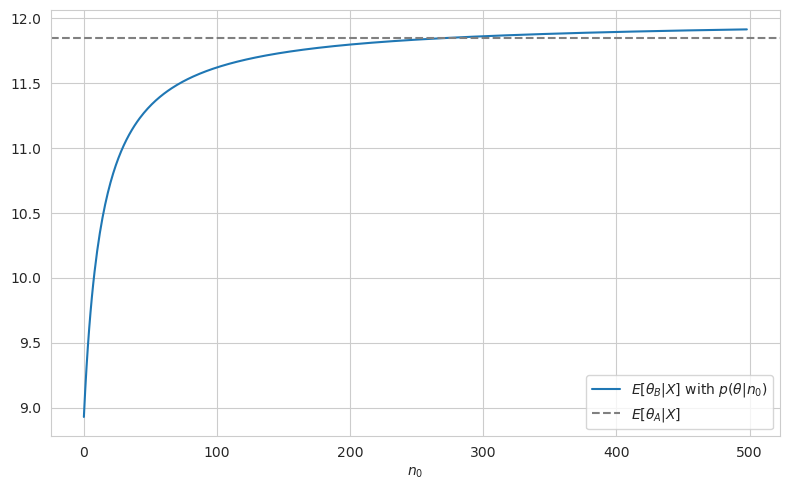
\includegraphics[width=0.8\textwidth]{3.3.b.png}
  \captionsetup{justification=centering}
  \caption{$\theta_B$ sensitivity to $n_0$}
\end{figure*}

\paragraph{(c)}
The dependency between $\theta_A$ and $\theta_B$ is worth considering, and it mostly has to do with the
relationship between the two strains. It is better to consult an expert on this matter. Then we can decide
whether the independence assumption makes sense or not. 
\newpage

\section{Excerise PH 3.5}
\paragraph{(a)}
As long as we model both the sampling distribution and the prior all within the exponential family, the resulting
posterior is also an exponential family distribution. The derivation also generalizes to priors that are
a mixture of distributions from the exponential family. The resulting posterior is simply a weighted sum
of each prior $p(\phi)$ that is updated by the data $Y$ separately.
\begin{proof}
\begin{align*}
  p(y|\phi) &= h(y)c(\phi)e^{\phi t(y)} \\
  p(Y|\phi) &= \prod_{i=1}^{n} h(y_i)c(\phi)e^{\phi t(y_i)} && Y_{i \in n} \overset{iid}{\thicksim} p(y|\phi) \\
    &\propto {c(\phi)}^{n} \exp(\phi \sum_{i=1}^{n} t(y_i)) \\
  \tilde{p}(\phi) &= \sum_{k=1}^{K} w_k p_k(\phi) && p(\phi) = \kappa(n_0, t_0) {c(\phi)}^{n_0} e^{n_0 t_0 \phi}
\end{align*}

\begin{align*}
  p(\phi|Y) &\propto p(Y|\phi)\tilde{p}(\phi) \\
    &\propto {c(\phi)}^{n} \exp(\phi \sum_{i=1}^{n} t(y_i)) \sum_{k=1}^{K} w_k {c(\phi)}^{n_0^{(k)}} \exp(n_0^{(k)} t_0^{(k)} \phi) \\
    &\propto \sum_{k=1}^{K} w_k {c(\phi)}^{n_0^{(k)} + n} \exp(\phi \times (n_0^{(k)} t_0^{(k)} + \sum_{i=1}^{n} t(y_i))) \\
    &\propto \sum_{k=1}^{K} w_k p_k(\phi | n_0^{(k)}+n, n_0^{(k)} t_0^{(k)} + n \overline{t}(Y))
\end{align*}
\end{proof}

\paragraph{(b)}
First we write the Poisson distribution in its exponential family form as below.
\begin{align*}
  p(y|\theta) &= \frac{1}{y!} \theta^y e^{-\theta} \thicksim Poission(\theta) \\
    &\propto \theta^y e^{-\theta} \\
    &= e^{y \log(\theta)} e^{-\theta} \\
    &= \exp[y\log(\theta) - e^{\log(\theta)}] \\ \\
  \therefore
    & \phi = \log(\theta) \\
    & c(\phi) = \exp({A(\phi)}^{-1}) = \exp(e^{-\phi}) \\
    & t(y) = y \\ \\
  p(y|\phi) &\propto \exp(e^{-\phi}) e^{\phi y}
\end{align*}
Hence, its conjugate prior Gamma has the form of $Gamma(\phi|n_0, t_0) = p(\phi) \propto \exp(n_0 e^{-\phi}) e^{n_0 t_0 \phi}$.
And the posterior distribution is
\begin{align*}
  p(\phi|Y) &\propto \sum_{k=1}^{K} w_k \exp((n_0^{(k)}+n) e^{-\phi}) \exp((n_0^{(k)} t_0^{(k)} + n\overline{y}) \times \phi) \\
  where \,\, \overline{y} &= \frac{1}{n} \sum_{i=1}^{n} y_i
\end{align*}


\section{Excerise PH 3.8}
\newpage


\section{Excerise PH 4.3}
\paragraph{(a)}
Overall the Poisson generative model matches quite well with the data, $Y_A$. 

\begin{figure*}[!h]
  \centering
  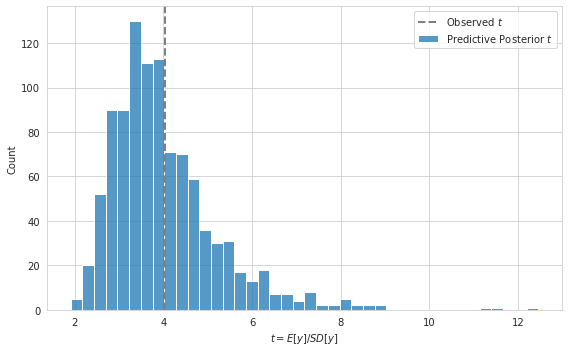
\includegraphics[width=0.8\textwidth]{4.3.a.png}
  \captionsetup{justification=centering}
  \caption{Posterior Predictive Model Check for Group A}
\end{figure*}

\paragraph{(b)}
However, the model does not work well with the group B data, $Y_B$. It could be that we have a terrible prior,
not enough data size, or perhaps Poisson is just not a good model for the data.

\begin{figure*}[!h]
  \centering
  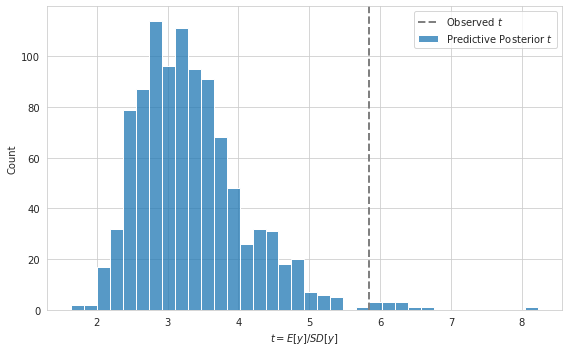
\includegraphics[width=0.8\textwidth]{4.3.b.png}
  \captionsetup{justification=centering}
  \caption{Posterior Predictive Model Check for Group B}
\end{figure*}
\newpage


\section{Excerise 5}
\paragraph{(a)}
Given the prior $\theta \thicksim Gamma(a=10, b=1)$ and the sampling model
$X_{i \in n} \overset{iid}{\thicksim} Poisson(\theta)$, the posterior is also a gamma distribution.
Now we know we received a total of 200 call from 10 different days, the Posterior
\[ \theta|\mathbf{X} \thicksim Gamma(a=210, b=11) \]
The $\theta$ estimate that minimizes the L2 loss is the mean, 19.09. And the $\theta$ estimate
that minimizes the L1 loss is the median, 19.06.

\paragraph{(b)}
The model is reasonable because observing 20 calls on average is a typical belief shown in the posterior.
However, given only one data point, it is hard to tell the truth. The underlying data points might well be
$\{0, 0, \dots, 0, 200\}$. In such a case, our model performs poorly instead. In other words, if all we
care about is the average, the model is fine.

\begin{figure*}[!h]
  \centering
  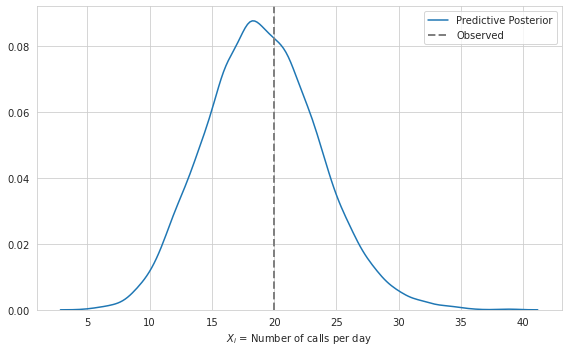
\includegraphics[width=0.8\textwidth]{5.b.png}
  \captionsetup{justification=centering}
  \caption{Posterior Predictive Model Check}
\end{figure*}
\newpage

\end{document}